%\documentclass[dvipdfmx]{beamer}      % platex の場合
\documentclass[handout]{beamer}        % lualatex の場合
\usepackage{mySld}

\begin{document}
\title{基礎コンピュータ工学\\第3章 組み立て\\(パート4)}
\date{}

\begin{frame}
  \titlepage
  \centerline{\url{https://github.com/tctsigemura/TecTextBook}}
  \vfill
  \centerline{本スライドの入手:
    \raisebox{-7mm}{
\includegraphics[scale=0.3]{../Img/QRs3_4.png}}}
\end{frame}

%==============================================================================
%\begin{frame}
%  \frametitle
%  \tableofcontents
%\end{frame}

\section{組み立て}
%==============================================================================
\begin{frame}
  \frametitle{ゴム足の取り付け}
  \vfill
  \centerline{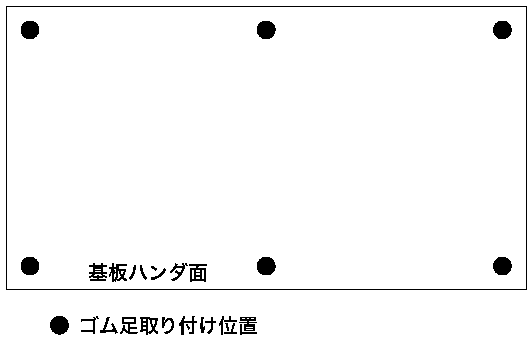
\includegraphics[scale=0.7]{../Tikz/asi.pdf}}
  \vfill
  \begin{enumerate}
    \item[1.] 基板の取り付け位置を確認する.
    \item[2.] アルコールで取り付け位置を周辺を拭く.
    \item[3.] 部品から鉄板とシールを剥がす.
    \item[4.] 両面テープで貼り付ける.
  \end{enumerate}
  \vfill
\end{frame}

%==============================================================================
\begin{frame}
  \frametitle{プッシュスイッチの頭の取り付け}
  \vfill
  \centerline{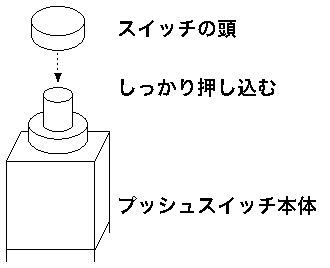
\includegraphics[scale=0.8]{../Tikz/atama.pdf}}
  \vfill
  \begin{enumerate}
    \item[1.] しっかり押し込む.
    \item[2.] 全てのプッシュスイッチに取り付けたか?
  \end{enumerate}
  \vfill
\end{frame}

%==============================================================================
\begin{frame}
  \frametitle{完成}
  \begin{enumerate}
    \item[1.] 命令表をケース蓋の裏側に貼り付ける.
    \item[2.] チェックリスト(ハンダ付け後の確認)に従い部品を再度確認する.
    \item[3.] 設計データの書き込みをしてもらう.
    \item[4.] チェックリスト(動作試験)に従い操作できるか確認する.
    \item[4.] 操作の練習のため,オルゴールのデータ打ち込みをやってみる.
  \end{enumerate}
  \vfill
\end{frame}

%==============================================================================
%\begin{frame}
%  \frametitle{}
%\end{frame}

\end{document}
